\documentclass[12pt]{report}

\usepackage{times}
\usepackage{float}
\usepackage{xcolor}
\usepackage{dirtree}
\usepackage{graphicx}
\usepackage{hyperref}
\usepackage{indentfirst}
\usepackage[margin=1in]{geometry}

\hypersetup{colorlinks=true, linkcolor=teal}
\setlength{\DTbaselineskip}{25pt}
\renewcommand{\DTstyle}{\rmfamily\large}

\newcommand{\n}{\par}
\newcommand{\br}{\n\vspace{1 em}\n}

\title{SBA Web Application Report}
\author{David W.}
\date{Last Revised \today}

\begin{document}
\maketitle

\textbf{Introduction}
\br
This report discusses Assignee, a web application developed to fulfill the SBA task of implementing an assignment system.
\br
This report includes the following chapters on various aspects:
\begin{itemize}
	\item \S{} \hyperref[overview]{Overview}:\\
	      Project objectives and structure;
	\item \S{} \hyperref[data-layer]{Data Layer}:\\
	      Relational database design and implementation;
	\item \S{} \hyperref[application-layer]{Application Layer}:\\
	      Design and implementation of site backend components;
	\item \S{} \hyperref[presentation-layer]{Presentation Layer}:\\
	      Design and implementation of site frontend components;
	\item \S{} \hyperref[security]{Security}:\\
	      User authentication and cross-layer interaction security;
	\item \S{} \hyperref[accessibility]{Accessibility}:\\
	      Considerations for site accessibility and localization (l10n);
	\item \S{} \hyperref[performance]{Performance}:\\
	      Optimizations for application performance;
	\item \S{} \hyperref[quality-assurance]{Quality Assurance}:\\
	      Unit and integration testing;
	\item \S{} \hyperref[tools-used]{Tools Used}:\\
	      Applications, extensions, packages, and libraries utilized during development;
\end{itemize}
\tableofcontents




\chapter{Overview} \label{overview}



\section{Project Objectives} \label{overview.project-objectives}
The following pages provide a brief overview of user capabilities by role.
We have three core systems - User, Team, and Assignment - designed to manage complex application logic, as detailed below
\footnote{Only workflow-related points are included; GUI aspects are excluded.
	Each task is described broadly (e.g., login), with detailed information provided later in the report.}
\footnote{Symbolic notes:\n
	...... $\rightarrow$ \{A\}: The user performing the action attains role A.\n
	\{B\} $\rightarrow$ \{C\}: The action allows a user with role B to attain role C.\n
	\{D\} $\in$ \{E\}: Role D inherits from role E, granting users with role D all permissions of role E.}.

\subsection{User System} \label{overview.project-objectives.user-system}
Roles: \{Site Visitors\}, \{Logged-in Users\}\n
\begin{itemize}
	\item \{Site Visitors\}
	      \begin{itemize}
		      \item Register for accounts;\null\hfill $\rightarrow$ \{Logged-in Users\}
		      \item Log in to existing accounts;\null\hfill $\rightarrow$ \{Logged-in Users\}
	      \end{itemize}
	\item \{Logged-in Users\}
	      \begin{itemize}
		      \item Change password;
		      \item Change username or email;
		      \item Modify other settings;
		      \item Log out;\null\hfill $\rightarrow$ \{Site Visitors\}
		      \item Delete account;\null\hfill $\rightarrow$ \{Site Visitors\}
	      \end{itemize}
\end{itemize}\n
The User System is a standard account management system found in web applications.
It allows visitors to create accounts, while registered users can log in and manage their account settings.
\br
Authentication techniques are implemented to support this system, with detailed information provided in later chapters.
\br
The User System is central to all components of this application,
including the \S{} \hyperref[overview.project-objectives.team-system]{Team System},
the \S{} \hyperref[overview.project-objectives.assignment-system]{Assignment System},
and any future systems that may be introduced,
such as a Posts and Comments System or an Instant Messaging System using P2P WebRTC or C/S WebSockets.


\subsection{Team System} \label{overview.project-objectives.team-system}
Roles: \{Users\}, \{Team Members\}, \{Team Monitors\}, \{Team Owners\}\n
\begin{itemize}
	\item \{Users\}
	      \begin{itemize}
		      \item Join teams;\null\hfill $\rightarrow$ \{Team Members\}
		      \item Create teams;\null\hfill $\rightarrow$ \{Team Owners\}
	      \end{itemize}
	\item \{Team Members\} $\in$ \{Users\}
	      \begin{itemize}
		      \item Leave the team;\null\hfill $\rightarrow$ \{Users\}
		      \item Comment on messages*;
	      \end{itemize}
	\item \{Team Monitors\} $\in$ \{Team Members\}
	      \begin{itemize}
		      \item Invite team members;\null\hfill \{Users\} $\rightarrow$ \{Team Members\}
		      \item Kick team members;\null\hfill \{Team Members\} $\rightarrow$ \{Users\}
		      \item Post messages*;
	      \end{itemize}
	\item \{Team Owners\} $\in$ \{Team Monitors\}
	      \begin{itemize}
		      \item Change team name;
		      \item Change team description;
		      \item Appoint team monitors;\null\hfill \{Users\} $\rightarrow$ \{Team Monitors\}
		      \item Remove team monitors;\null\hfill \{Team Monitors\} $\rightarrow$ \{Users\}
		      \item Delete the team;\null\hfill $\rightarrow$ \{Users\}
	      \end{itemize}
\end{itemize}\n
Similar to Google Classroom, users can create or join teams,
with team owners having the ability to appoint or remove team monitors to assist in managing the team.
Additionally, roles within the hierarchy can manage members and perform team actions to varying degrees and extents.
\br
The *post and comment features are not implemented in the initial version of the web app, as they are considered a lower priority.
If these features are added later, they will be decoupled from the current system.
\br
The Team System is central to the \S{} \hyperref[overview.project-objectives.assignment-system]{Assignment System}.


\subsection{Assignment System} \label{overview.project-objectives.assignment-system}
Roles: \{Team Owners\}, (\{Team Members\},) \{Assignees\}\n
\begin{itemize}
	\item \{Team Owners\}
	      \begin{itemize}
		      \item Author assignments;
		      \item Add attachments to assignments;
		      \item Assign assignments;\null\hfill \{Team Members\} $\rightarrow$ \{Assignees\}
		      \item Revoke assignments;\null\hfill \{Assignees\} $\rightarrow$ \{Team Members\}
		      \item Grade, comment on, and return submissions;
	      \end{itemize}
	\item \{Assignees\} $\in$ \{Team Members\}
	      \begin{itemize}
		      \item Submit assignments;
		      \item Add attachments to submissions;
	      \end{itemize}
\end{itemize}\n
The Assignment System is the core feature we are tasked with completing. The system operates intuitively:\n
Team owners can assign assignments to selected team members with a deadline.
Assignees can draft and submit their work.
After submission, the team owner can grade the assignment, provide comments, and return it to the assignee.
\br
An attachment system is designed to manage attachment files,
enabling team owners and assignees to add additional files to their assignments and submissions without needing to reattach all previous files after exiting.
More details will be provided in later chapters.



\section{Miscellaneous} \label{overview.miscellaneous}


\subsection{Folder Structure} \label{overview.project-structure.folder-structure}
To maintain a clear separation of concerns and promote modularity, the web application is divided into three layers,\n
Data Layer: Manages data storage and retrieval;\n
Application Layer: Contains the business logic and processes data;\n
Presentation Layer: Handles user interface and user interaction;
\br
This organization can be observed in the project folder structure.
While the folder structure may undergo frequent changes, its fundamental layout will remain consistent across revisions.
\newpage
\begin{figure}[h!]
	\centering
	\begin{minipage}{0.3\linewidth}
		\dirtree{%
			.1 /.
			.2 report/.
			.2 database/.
			.2 site/.
			.3 backend/.
			.3 frontend/.
		}
	\end{minipage}
	\caption{Overall Folder Structure}
	\label{fig:overview-folder-structure}
\end{figure}
The report/ directory contains the \LaTeX{} source of the report, media assets used in the report, and other related documents.
\br
The database/ directory corresponds to the Data Layer.
It is located under design/ because the hosted database is independent of the site/ folder (linked only via the database URL in the .env file).
Only the distribution .sql file used to instantiate the database is stored here.
Further details can be found in the chapter \S{} \hyperref[data-layer]{Data Layer}.
\br
The directory backend/ corresponds to the Application Layer.
Further details can be found in the chapter \S{} \hyperref[application-layer]{Application Layer}.
\br
The directory frontend/ corresponds to the Presentation Layer.
More information is provided in the chapter \S{} \hyperref[presentation-layer]{Presentation Layer}.


\subsection{Repository} \label{overview.project-structure.repository}
The entire project folder is hosted in a repository available at
\href{https://github.com/CarbonicSoda/assignee}{GitHub/CarbonicSoda/assignee}
\footnote{Refer to github.com/CarbonicSoda/assignee.}
for inspection.
\br
With GitHub, we can review all past commits from the start of this project to the latest update or patch.
This functionality not only facilitates version control and debugging but also enables simultaneous work on the back-end and front-end through branching.




\chapter{Data Layer} \label{data-layer}
This chapter covers the design and implementation of the supporting relational database.
\br
In \S{} \hyperref[data-layer.design]{Design},
we discuss the design of tables, fields, and their data types, along with the rationales behind these choices.
We also explore the relational mappings of tables and fields from multiple perspectives.
Finally, we will delve into the adoption of normal forms in greater detail.\n
In \S{} \hyperref[data-layer.implementation]{Implementation},
we will cover the actual deployment details of the database schema.



\section{Design} \label{data-layer.design}
The design of the relational database follows the blueprint outlined in the section \S{} \hyperref[overview.project-objectives]{Project Objectives}.
The three core systems and their related entities (roles) are utilized to structure and populate the database.
\br
Throughout the database, snake\_case is used for table and field names, in contrast to conventional practices of using CONSTANT\_CASE.
This choice helps distinguish entities from SQL commands, which are typically written in uppercase.


\subsection{User System} \label{data-layer.design.user-system}
The User System serves as the backbone of the entire web application, responsible for storing user account-related data.
This system encompasses user identifiers, authentication data and user preferences.
\br
The User System consists of five tables, as described below,
\begin{itemize}
	\item users: Contains user account identification information;
	\item authcodes: Holds user email authentication codes;
	\item passwords: Manages user password information;
	\item sessions: Tracks user browser sessions;
	\item preferences: Stores user preferences;
\end{itemize}
Relations:\n
A \{user\} can only have a single valid email \{authcode\} at a time;\null\hfill (Optional)\n
An email \{authcode\} is for one \{user\} only;\null\hfill (Mandatory)
\br
A \{user\} can only have a single \{password\};\null\hfill (Mandatory)\n
A \{password\} is for a single \{user\};\null\hfill (Mandatory)
\br
A \{user\} can have many \{sessions\} at the same time;\null\hfill (Optional)\n
A \{session\} is borne by one \{user\} only;\null\hfill (Mandatory)
\br
A \{user\} can only have a single set of \{preferences\};\null\hfill (Mandatory)\n
A set of \{preferences\} is owned by a single \{user\};\null\hfill (Mandatory)
\begin{figure}[h!]
	\centering
	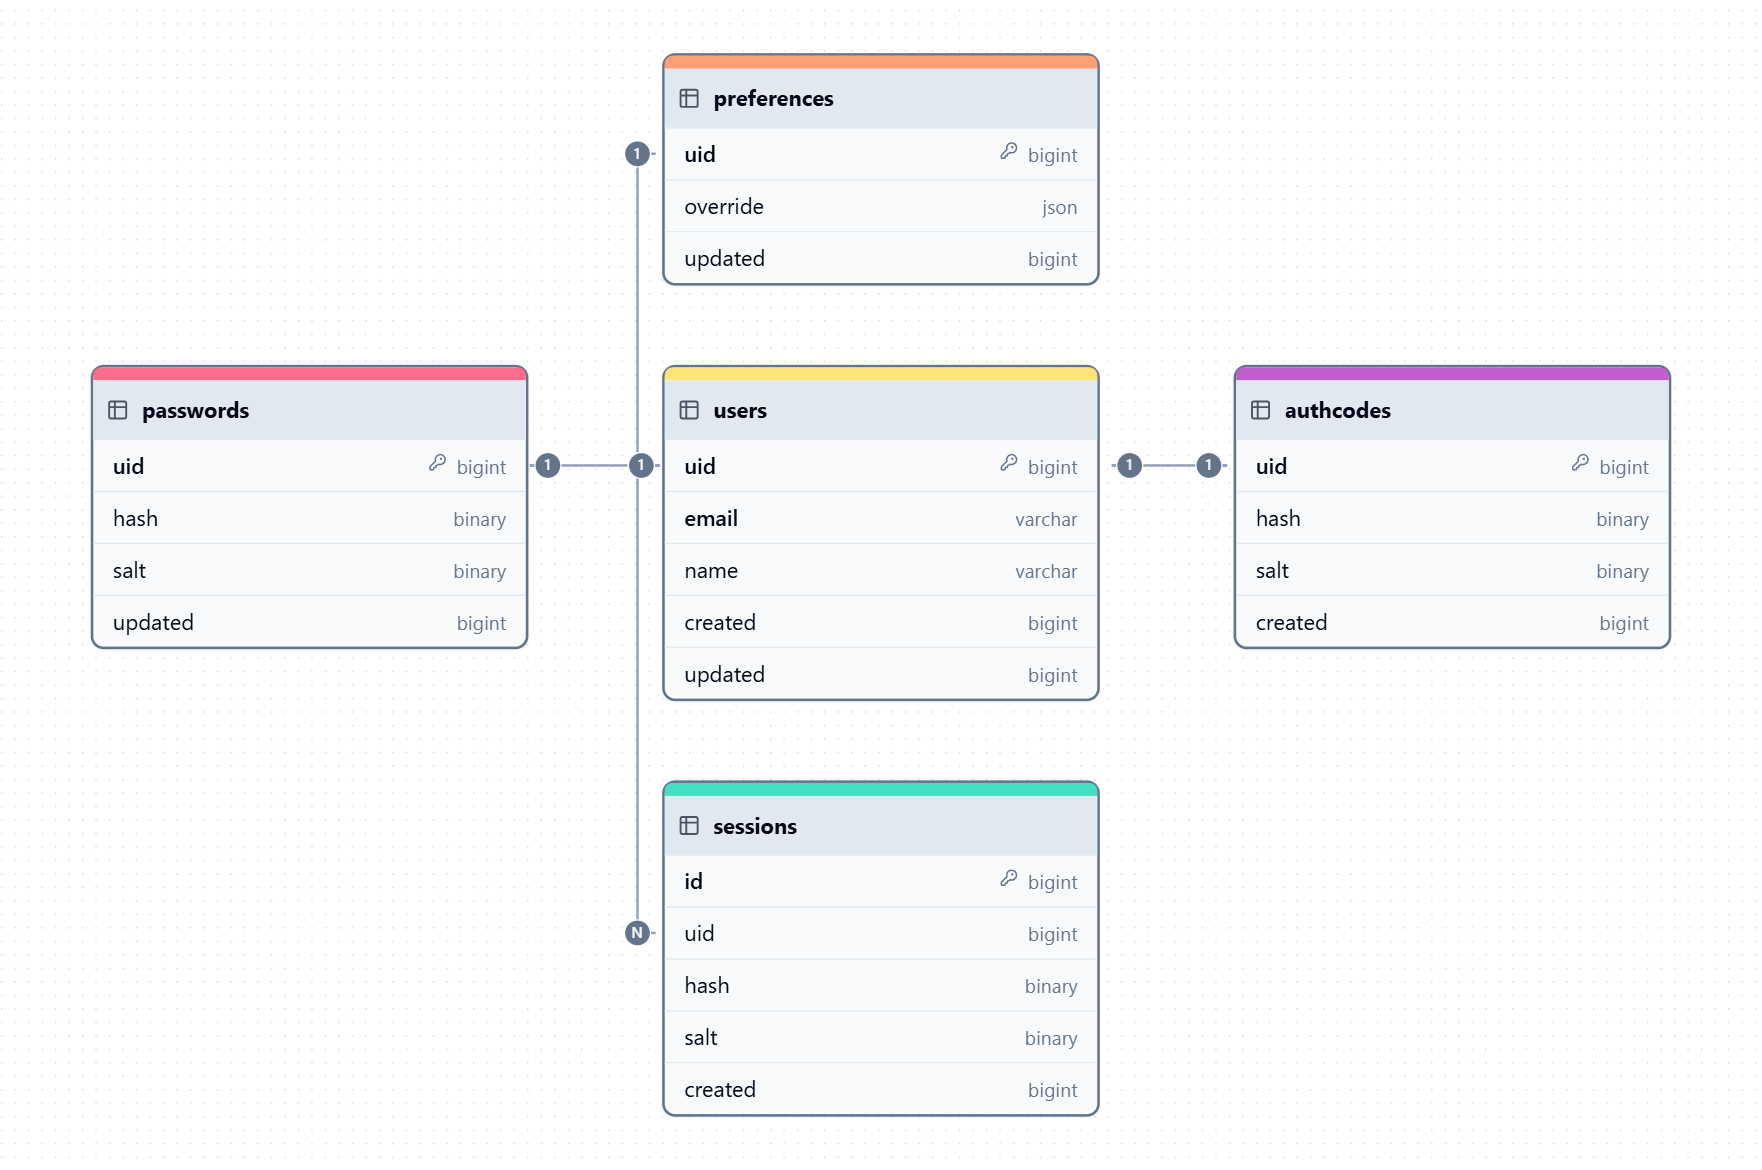
\includegraphics[width=1\linewidth]{user_system.jpeg}
	\caption{User System ER Diagram}
	\label{fig:user-system-er}
\end{figure}
\br
When not otherwise specified (Null-able), all table attributes are defined as Not Null.
This approach is taken to prevent potential issues related to database consistency that can arise from having Null entries.
It reduces the risk of anomalies and simplifies backend application logic dealing with complicated queries.
\br
Rationales and more details on table fields are given below.\n

\subsubsection{Table - users} \label{data-layer.design.user-system.users}
In Assignee, users can register for accounts using their email addresses.
The email address acts as the unique identifier for user login.
This approach simplifies the process, eliminating the need for users to create a username,
as their email is readily available for use.\n
While logging in with their email addresses, users can choose their own display names for better identification.
These display names do not need to be unique, allowing users the flexibility to select names that resonate with them.
\begin{itemize}
	\item uid (Unsigned BIGINT) (Auto-Increment) (Primary Key)\n
	      Although \{email\} is a candidate key for the table, \{uid\} is chosen as the primary key for several reasons:\n
	      \begin{itemize}
		      \item Storage Efficiency: Tables referencing a user can save on storage space by using a BIGINT instead of a VARCHAR.
		      \item Indexing Performance: Indexing this frequently accessed table is typically faster with a BIGINT.
		      \item Consistency and Flexibility: Using an auto-increment primary key helps maintain data\-base consistency and flexibility, especially if there comes a time when email login is no longer used.
	      \end{itemize}\n
	      BIGINT is set to be unsigned to maintain consistency across the application.
	      This approach prevents potential issues in backend logic that could arise from wrapped negative numbers,
	      ensuring stability and reliability in data handling.
	\item email (ASCII VARCHAR(254)) (Unique)\n
	      The email address used for account registration and login is defined as VARCHAR type in the database schema, necessarily unique.
	      This choice accommodates the flexible length of email addresses.\n
	      VARCHAR is capped to 254 characters in ASCII, this is to align with the standards outlined in
	      \href{https://www.rfc-editor.org/rfc/rfc5322}{RFC 5322: Internet Message Format}
	      \footnote{Refer to www.rfc-editor.org/rfc/rfc5322.}.
	\item name (UTF-8 VARCHAR(30))\n
	      The arbitrary display name users may use.
	      It is of UTF-8 encoding to encompass usernames in different languages or even emojis.
	      Capped to 30 characters, this ensures the username will not be too long for display yet not too short for personalization.
	\item created \& updated (Unsigned BIGINT)\n
	      Metadata fields for table. They record the time the entry is created / updated.\n
	      Instead of DATETIME or TIMESTAMP, 64-bit BIGINT is used for several reasons:
	      DATETIME is dependent on the database used, i.e. MySQL and might not be cross-database compatible.
	      TIMESTAMP stores \href{https://en.wikipedia.org/wiki/Unix_time}{UNIX Timestamps}
	      \footnote{Refer to en.wikipedia.org/wiki/Unix\_time.}
	      which is indeed what we want to store,
	      but is signed 32-bit integer in MySQL and is thus prone to the
	      \href{https://en.wikipedia.org/wiki/Year_2038_problem}{Y2K38 Problem}
	      \footnote{Refer to en.wikipedia.org/wiki/Year\_2038\_problem.}.
	      By using middlewares in backend API handling this problem can be mitigated.
	      Details in \S{} \hyperref[application-layer.design.middlewares]{Middlewares}.
	      BIGINT is unsigned since all timestamps that could exist in the database would be after the Unix epoch.
	      The attribute(s) also exist in other tables, unless something is special about it, they will not be otherwise mentioned.
\end{itemize}

\subsubsection{Table - authcodes} \label{data-layer.design.user-system.authcodes}
Upon user registration or log-in (contexts that require better authentication) an authcode would be sent via email.
(Or phone just in case email login is no longer used, this is an example of the benefit of using \{uid\} as primary key for \{users\})
\begin{itemize}
	\item uid (Unsigned BIGINT) (Primary Key) (Foreign Key $\rightarrow$ users.uid)\n
	      Only a single email authcode would be valid for a user at a time,
	      before sending a new authcode in backend the old one (if exists) would be deleted.
	      Therefore, uid is sufficiently unique as the primary key of the table.\n
	      There will be a \href{https://en.wikipedia.org/wiki/Cron}{Cron Job}
	      \footnote{Refer to en.wikipedia.org/wiki/Cron.}
	      to remove expired authcodes from the database,
	      with expiry calculated with \{created\} + \{Some Time e.g. 10 minutes\},
	      in interval of an hour or alike defined in backend.
	      When a user attempts to use an authcode, the backend will also check if it expired.\n
	      The relation mapping between \{authcodes\} and \{users\} has ON DELETE: CASCADE,
	      which will remove all entries in \{authcodes\} with authcodes.uid = users.uid upon deletion of a \{users\} entry automatically,
	      preventing anomalies on entry deletion.
	      This together with ON UPDATE: RESTRICT, which restricts updating referenced field,
	      is applied to all relations in the database and will not be mentioned again otherwise.
	\item hash (BINARY(32)) \& salt (BINARY(16))\n
	      Storing authentication related information in raw form is not a good idea, i.e. password or authcode.
	      Instead, the raw data is hashed using
	      \href{https://en.wikipedia.org/wiki/Cryptographic_hash_function}{Cryptographically Secure Hashing Algorithms}
	      \footnote{Refer to en.wikipedia.org/wiki/Cryptographic\_hash\_function.}
	      and stored in digest form.
	      Hashes are practicably impossible to crack reversely in reasonable polynomial time.
	      On attempt to verify input data, it is hashed again with the same algorithm and compared with the stored hash.\n
	      The only reason the hash is stored in BINARY is that the algorithm used returns a byte buffer directly, and it is simply more convenient to do so.
	      A variable digest length hashing function
	      \href{https://keccak.team/kangarootwelve.html}{K12}
	      \footnote{Refer to keccak.team/kangarootwelve.html.}
	      is used instead of traditional SHA-256, which is weaker than K12 in cryptanalysis.\n
	      However, storing only the hash is vulnerable to
	      \href{https://en.wikipedia.org/wiki/Rainbow_table}{Rainbow Table Attacks}
	      \footnote{Refer to en.wikipedia.org\-/wiki/Rainbow\_table.},
	      thus a salt is needed. A salt is a BINARY generated with a
	      \href{https://en.wikipedia.org/wiki/Cryptographically_secure_pseudorandom_number_generator}{Cryptographically Secure Pseudorandom Number Generator}
	      \footnote{Later abbreviated as CSPRNG.\n
		      Refer to en.wikipedia.org/wiki/Cryptographically\_secure\_pseudorandom\_number\_generator.}
	      with enough entropy, that is concatenated to the raw string (in byte buffer form) before hashing.
	      It is of length 16 bytes in our case which is totally sufficient for the purpose.
	      The salt will be stored directly in the database along with the hash,
	      as having the salt will not provide any help in attempt to crack the original string.\n
	      To summarize, given a raw string as input, a random salt of 16 bytes would be generated,
	      appended to the raw string after converting it into byte form.
	      After which the resulting byte buffer is hashed with K12 into a 256-bits digest and stored in the database together with the salt.
	      When a user attempts to verify his input against the correct one,
	      his input would be appended with the salt stored in the database and hashed with K12 again,
	      to check if the resulting digest matches with the stored hash.\n
	      Technically there is a chance for hashes to collide with each other with different input,
	      but in the case of using a 32 bytes digest with salt in use, the chance would be vanishingly low
	      \footnote{The collision chance calculation method used in this report: \href{https://stackoverflow.com/a/62667633}{Probability of Hash Collision on StackOverflow}.\n
		      Refer to stackoverflow.com/a/62667633.}:
	      you would need roughly $10^{31}$ items before having an approximate $10^{-15}$ chance of collision even without salts.\n
	      Hash + salt is used in all authentication related tables in the database, and will not be detailed again otherwise.
	      However, more information could be found in
	      \S{} \hyperref[application-layer.implementation.authentication]{Application Layer - Authentication} and
	      \S{} \hyperref[security.authentication]{Security - Authentication}.
\end{itemize}

\subsubsection{Table - passwords} \label{data-layer.design.user-system.passwords}
\begin{itemize}
	\item uid (Unsigned BIGINT) (Primary Key) (Foreign Key $\rightarrow$ users.uid)\n
	      The uid of user that owns the password.
	\item hash (BINARY(32)) \& salt (BINARY(16))\n
	      Hash and salt of the user password.
	\item updated (Unsigned BIGINT)\n
	      Will also be used to track how long it was since the user last changed his password.
\end{itemize}

\subsubsection{Table - sessions} \label{data-layer.design.user-system.sessions}
To keep user logged-in in certain scenarios, browser sessions must be used.
Many browser sessions can exist at the same time for the same user.
When a user chose to stay logged-in, a bearer token of form
\{ uid: int, token: string \}
will be generated,
uid being the uid of the session bearer, and
token being a random binary number generated by a CSPRNG in hex representation.
The token will then be serialized and stored in the browser cookie for the site having an expiry date itself.\n
The hash will be created from a concatenation of (browser info + device info etc.) + token + salt.
Upon attempt to log in to a session,
for all sessions with sessions.uid = bearer\_token.uid,
expiry would be checked in backend with respect to \{created\}.
Then, if one is still active, the current browser info etc. would be retrieved and concatenated with bearer\_token.token,
hashed with salt and compared with the stored hash.
If matched, the user would be logged-in and handed a new bearer token (old one would be deleted), renewing session expiry.\n
Also, the validity of the token will be verified for further actions upon any CRUD API requests and on periodic checks.
More details will be handed in \S{} \hyperref[application-layer.implementation.authentication]{Application Layer - Authentication} and
\S{} \hyperref[security.authentication]{Security - Authentication}.
\begin{itemize}
	\item uid (Unsigned BIGINT) (Primary Key) (Foreign Key $\rightarrow$ users.uid)\n
	      The uid of the session bearer.
	\item hash (BINARY(32)) \& salt (BINARY(16))\n
	      Hash and salt of the reinforced session token.
\end{itemize}

\subsubsection{Table - preferences} \label{data-layer.design.user-system.preferences}
\begin{itemize}
	\item uid (Unsigned BIGINT) (Primary Key) (Foreign Key $\rightarrow$ users.uid)\n
	      The uid of the user that has the preferences.
	\item override (\href{https://dev.mysql.com/doc/refman/9.2/en/json.html}{JSON}
	      \footnote{Refer to dev.mysql.com/doc/refman/9.2/en/json.html.}
	      \footnote{JSON is supported by all major DBMS nowadays. If somehow not, JSON could be easily serialized into string and stored instead.})\n
	      The user would be allowed to override default settings and the overridden ones would be specified in this JSON object.
	      For instance, if the default settings are \{ a: 1, b: \{ c: true \}, d: "h" \},
	      and the user only alters settings.b.c, the JSON object would be like \{ b: \{ c: false \} \}.\n
	      This is against 1NF (actually it might not be, as argued below) in return of way greater flexibility and storage efficiency.
	      Imagine a few other settings are added, a table in 1NF would need more columns to deal with this.
	      However with our methodology, upon addition of new settings, they would automatically be the default values waiting for the user to override.
	      Also, nesting settings would not have been possible in 1NF.
	      Only storing overridden settings will save a lot of storage space and is flexible in the long term.\n
	      It is worth mentioning that this may not be a violation of 1NF at all.
	      Scholar C. J. Date has argued that values can be arbitrarily complex objects
	      \footnote{Date, C. J. (2007). What First Normal Form Really Means.}.
	      But this is open to interpretations.
\end{itemize}

\subsubsection{Indexes} \label{data-layer.design.user-system.indexes}
Most of the tables in the User System have one-to-one relations with \{users\},
so would not need additional indexing.
However, \{sessions\} and \{users\} have a many-to-one relation.
To easily retrieve all sessions owned by a user, sessions.uid is indexed.\n
It is worth mentioning that unlike the obsolete binary search based index taught in textbooks, modern DBMS typically uses
\href{https://en.wikipedia.org/wiki/B-tree}{B-Trees}
\footnote{Refer to en.wikipedia.org/wiki/B-tree.}
for indexing, which is self-balancing.
That means, unlike binary search based indexes that would require rebuilding the index from scratch on insert / delete,
or BST-based indexes with $O(n)$ worst case time complexities for search / insert / delete,
it would only require at most $O(logn)$ in any scenario.
Implication is that in modern DBMS, indexes are way cheaper and the overhead of adding many indexes is staggeringly small.\n
Thus, in other systems that require more indexes, the trade-off of indexing would not be discussed as it is trivial.
Only the use case of the indexes would be covered otherwise.


\subsection{Team System} \label{data-layer.design.team-system}
The Team System is built upon the \S{} \hyperref[data-layer.design.user-system]{User System} to store teams related information.
This system contains team identification and invitation data,
whilst also keeping track of team monitor appointments.
\br
\begin{figure}[h!]
	\centering
	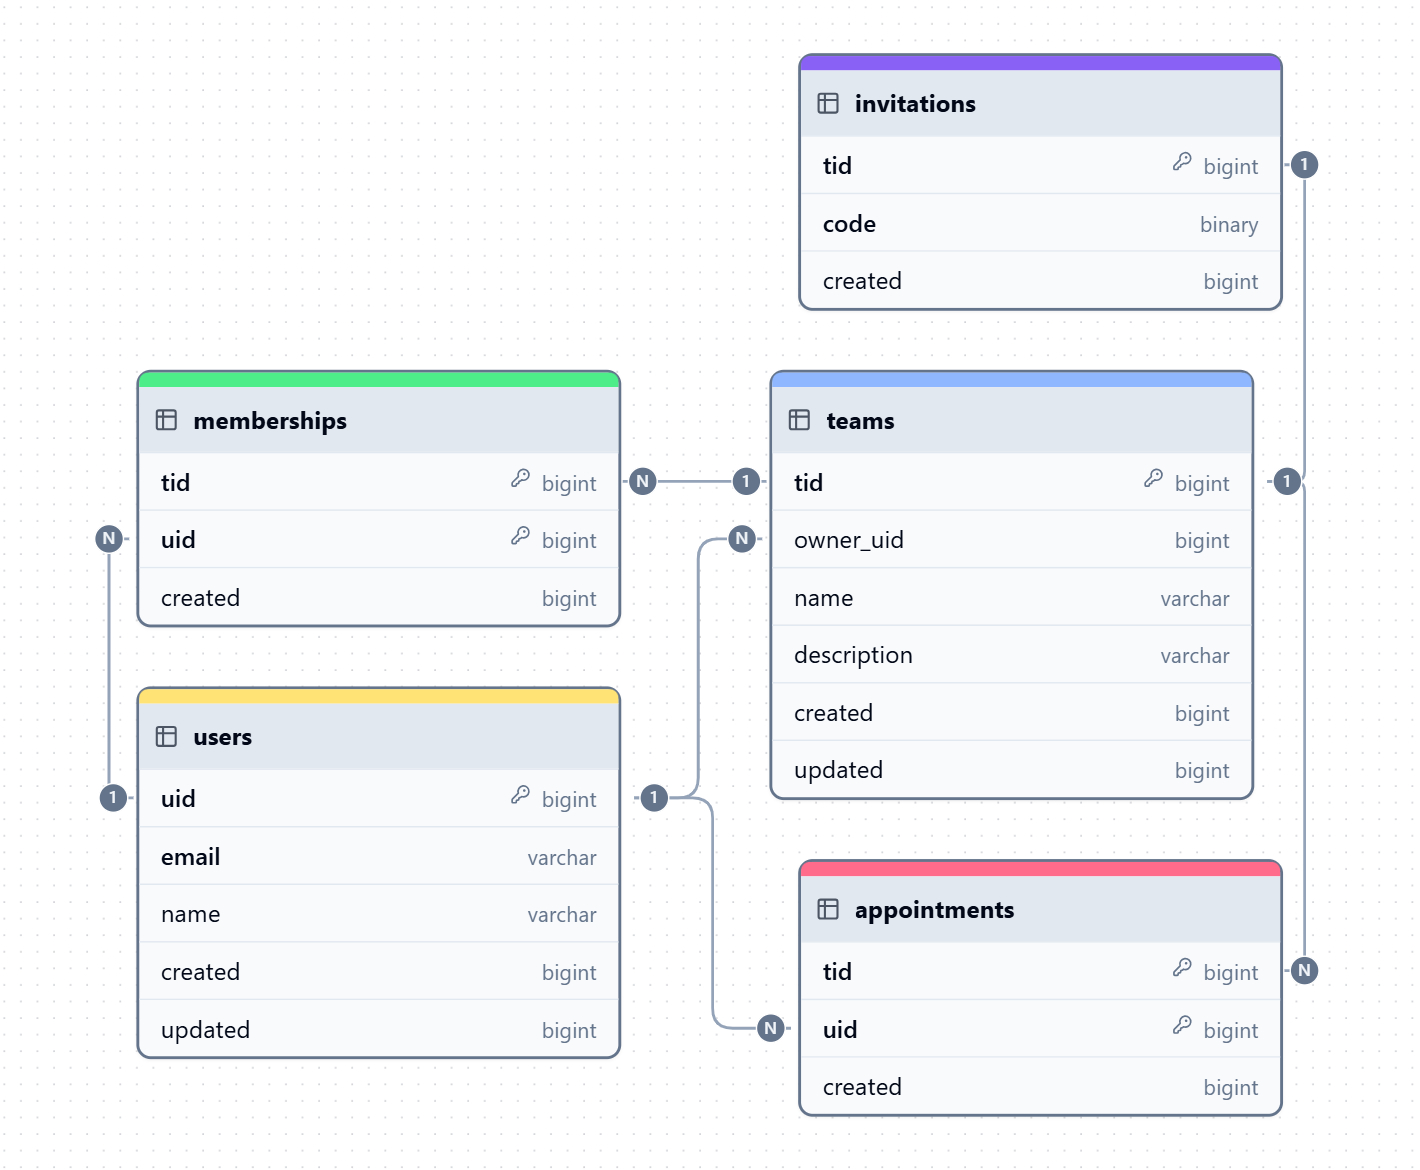
\includegraphics[width=1\linewidth]{team_system.jpeg}
	\caption{Team System ER Diagram}
	\label{fig:team-system-er}
\end{figure}
\br
The Team System encompasses five tables,
\begin{itemize}
	\item users: \S{} \hyperref[data-layer.design.user-system.users]{User System - users};
	\item teams: Contains team details;
	\item invitations: Holds team invitation codes;
	\item memberships: Stores user memberships of teams;
	\item appointments: Manages team monitor appointments;
\end{itemize}
\br
Table relations:\n
A \{user\} can create and own many \{teams\} at the same time;\null\hfill (Optional)\n
A \{team\} is owned by one \{user\} only;\null\hfill (Mandatory)
\br
A \{team\} can only have a single active \{invitation\} code;\null\hfill (Optional)\n
An \{invitation\} code is for a single \{team\};\null\hfill (Mandatory)
\br
A \{user\} can have many \{memberships\} at the same time;\null\hfill (Optional)\n
A \{membership\} is for a single \{team\} only;\null\hfill (Mandatory)
\br
A \{team\} can own many \{memberships\} at once;\null\hfill (Optional)\n
A \{membership\} is of one \{user\} only;\null\hfill (Mandatory)
\br
A \{user\} can be in many \{appointments\};\null\hfill (Optional)\n
An \{appointment\} is for a single \{team\} only;\null\hfill (Mandatory)
\br
A \{team\} can have many \{appointments\} at once;\null\hfill (Optional)\n
An \{appointment\} is of one \{user\} only;\null\hfill (Mandatory)
\br
Rationales and more details on table fields are given below.

\subsubsection{Table - users} \label{data-layer.design.team-system.users}
Refer to \S{} \hyperref[data-layer.design.user-system.users]{User System - users}.

\subsubsection{Table - teams} \label{data-layer.design.team-system.teams}
Users in assignee are allowed to create and own an arbitrary amount of teams.
This is slightly isomorphic to Google Classroom or Discord.
\begin{itemize}
	\item tid (Unsigned BIGINT) (Auto-Increment) (Primary Key)\n
	      Users should not have to waste time thinking of a unique team ID,
	      instead when they create a team an auto-increment tid would be given to the team,
	      and users may use whatever team name they want without worrying about uniqueness.
	\item owner\_uid (Unsigned BIGINT) (Foreign Key $\rightarrow$ users.uid)\n
	      The uid of the owner of the team.
	\item name (UTF-8 VARCHAR(30))\n
	      The arbitrary name of the team.
	      It is of UTF-8 encoding to support team names in different languages and emojis etc.
	      Capped to 30 characters ensures the team name will not be too long for display yet not too short for identification.
	\item description (UTF-8 VARCHAR(80))\n
	      The detailed description of the team displayed less prominently.
	      It is of UTF-8 encoding to support different languages and emojis etc.
	      Capped to 80 characters to promote clarity and facilitate display.
\end{itemize}

\subsubsection{Table - invitations} \label{data-layer.design.team-system.invitations}
Users can only become members of a team through invitations.
In assignee, invitations take the form of codes.
\begin{itemize}
	\item tid (Unsigned BIGINT) (Primary Key) (Foreign Key $\rightarrow$ teams.tid)\n
	      A team can only have one active invitation code at once.
	      Before getting a new invitation code, in backend the old one (if exists) would be deleted.
	      Therefore, tid is sufficiently unique as the primary key of the table.\n
	      There will be a cron job to remove expired invitation codes from the database,
	      with expiry calculated with \{created\} + \{Some Time e.g. 24 hours\},
	      in interval of a day or alike defined in backend.
	      When a user attempts to use an invitation code, the backend will also check if it expired.
	\item code (BINARY(4)) (Unique)\n
	      The invitation code will be generated with a CSPRNG even though security is less of a concern here.
	      The invitation code must be unique, the choice between tid and code as the primary key is minor,
	      as code will be indexed too.\n
	      For a randomly generated code to be unique, newly generated codes must be checked to not exist in the table already,
	      otherwise it would be regenerated. But this will not be a problem.
	      For one, the field is indexed, so uniqueness checks would be efficient;
	      For two, the chance of collision using a 4 bytes binary code is vanishingly low:
	      with $10,000$ codes in the table, a new code will only have a rough $0.01$ chance of colliding.
	      There must be approximately $100,000$ codes in the table before a collision must happen.
	      (Of course, if you deem that a small number,
	      making codes BINARY(5) would increase that number to $1,500,000$).\n
	      The code, when displayed in the application or inputted,
	      would be in hex representation e.g. A1B2FFCA.
	      A few good things about this is:
	      \begin{enumerate}
		      \item Easy to generate and transform;
		      \item Hex strings only have the characters 0-9 A-F, which will not be hard to distinguish, unlike 0 and O.
		            So they could be easily memorized;
	      \end{enumerate}
\end{itemize}

\subsubsection{Table - memberships} \label{data-layer.design.team-system.memberships}
A linking table for users' memberships in teams.
Users in assignee are allowed to join an arbitrary amount of teams and vice versa.
\begin{itemize}
	\item tid (Unsigned BIGINT) (Composite Primary Key) (Foreign Key $\rightarrow$ teams.tid)\n
	      The tid of the team that the membership involves.
	\item uid (Unsigned BIGINT) (Composite Primary Key) (Foreign Key $\rightarrow$ users.uid)\n
	      The uid of the user that is member of the involved team.
\end{itemize}

\subsubsection{Table - appointments} \label{data-layer.design.team-system.appointments}
A linking table for teams' monitor appointments.
Teams in assignee can appoint an arbitrary amount of teams monitors and vice versa.
\begin{itemize}
	\item tid (Unsigned BIGINT) (Composite Primary Key) (Foreign Key $\rightarrow$ teams.tid)\n
	      The tid of the team that appoints a team monitor.
	\item uid (Unsigned BIGINT) (Composite Primary Key) (Foreign Key $\rightarrow$ users.uid)\n
	      The uid of the appointed team monitor of the team.
\end{itemize}

\subsubsection{Indexes} \label{data-layer.design.team-system.indexes}
All foreign key fields are automatically indexed by MySQL.
Besides that, for tables with a composite primary key i.e. linking tables,
the proper subset of the composite key excluding the primary one will also be indexed.
For example, in \{memberships\}, the primary key index is (tid + uid).
This key can be used to speed up operations on (tid + uid) and \{tid\} alone,
as \{uid\} is only taken into consideration if \{tid\} is identical when sorting
\footnote{The order of keys in indexes does matter, but many ignore this fact.}.
However, \{uid\} alone cannot benefit from this index, and an additional index on \{uid\} must be added.
This way, no matter we are searching for a specific record, group by a team or group by a user,
an index will always be available at hand.\n
Also, unique fields are also indexed i.e. invitations.code for fast lookup and existence checks.
Otherwise, the foreign key indexes in the system are utilized for query grouping
\footnote{Indexes on foreign keys are mandatory in MySQL for optimization, here we discuss how they may be useful.},
e.g. index on teams.owner\_uid to retrieve all teams owned by a user.


\subsection{Assignment System} \label{data-layer.design.assignment-system}
The Assignment System is the core system supported by all previous systems.
This system tracks assignment details and attachments.
It also manages assignee submissions and attachments.
\br
The Assignment System contains six tables, as described below
\footnote{Only relations related to this system would be shown,
	e.g. users.uid - teams.owner\_uid will not be shown as it is irrelevant to assignments.}.
\begin{figure}[h!]
	\centering
	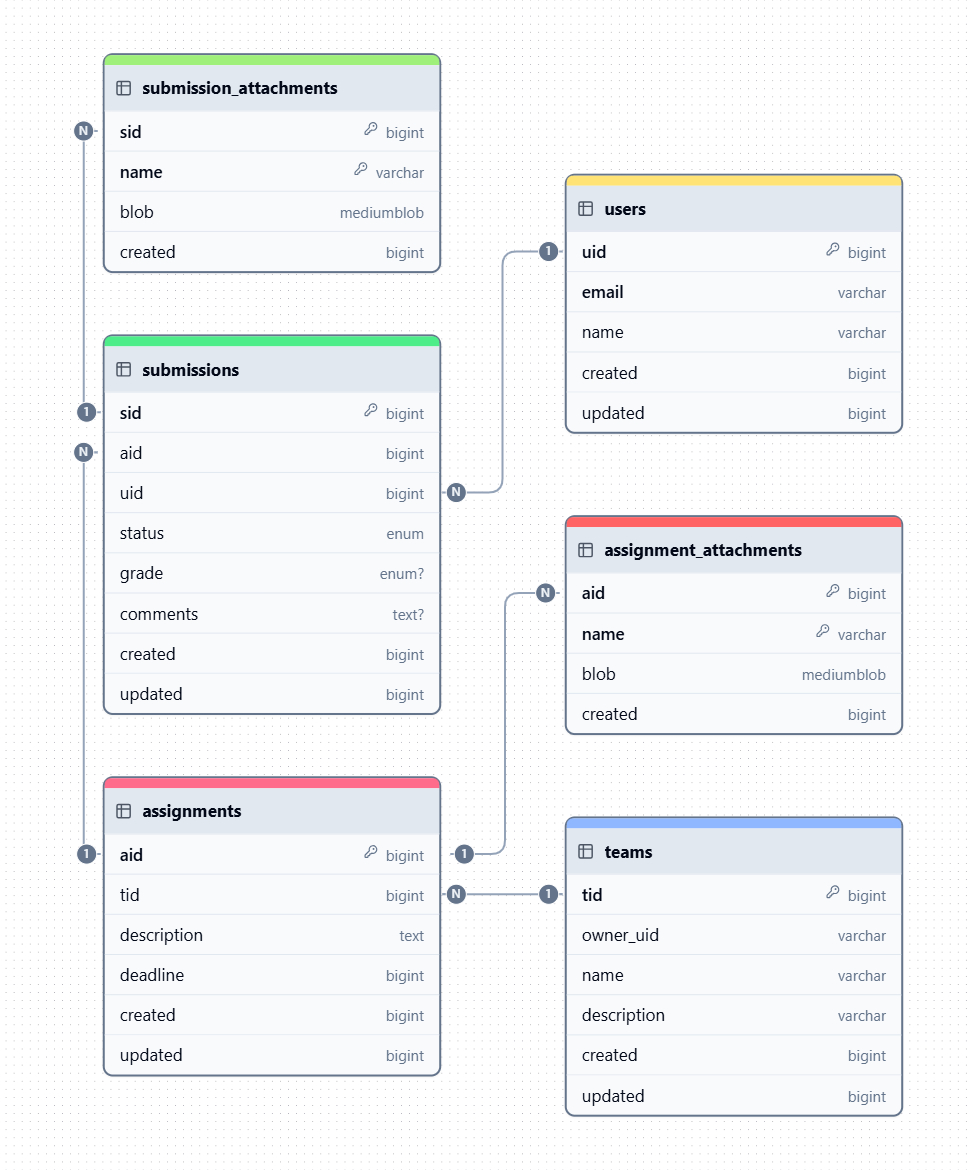
\includegraphics[width=1\linewidth]{assignment_system.jpeg}
	\caption{Assignment System ER Diagram}
	\label{fig:assignment-system-er}
\end{figure}
\begin{itemize}
	\item teams: \S{} \hyperref[data-layer.design.team-system.teams]{Team System - teams};
	\item assignments: Holds team assignment details;
	\item assignment\_attachments: Stores assignment attachments;
	\item users: \S{} \hyperref[data-layer.design.user-system.users]{User System - users};
	\item submissions: Manages assignee submission details;
	\item submission\_attachments: Contains submission attachments;
\end{itemize}
Relation mappings:\n
A \{team\} can post any amount of \{assignments\};\null\hfill (Optional)\n
An \{assignment\} is issued by a single \{team\};\null\hfill (Mandatory)
\br
An \{assignment\} may have many \{assignment\_attachments\};\null\hfill (Optional)\n
An \{assignment\_attachment\} is for a single \{assignment\};\null\hfill (Mandatory)
\br
An \{assignment\} can be assigned for many \{submissions\} (to assignees);\null\hfill (Optional)\n
A \{user\} can be assigned to many \{submissions\} (as assignee);\null\hfill (Optional)\n
A \{submission\} is only for one \{assignment\};\null\hfill (Mandatory)
\br
A \{submission\} may contain multiple \{submission\_attachments\};\null\hfill (Optional)\n
A \{submission\_attachment\} is only for one \{submission\};\null\hfill (Mandatory)
\br
They will be justified below.

\subsubsection{Table - teams} \label{data-layer.design.assignment-system.teams}
Refer to \S{} \hyperref[data-layer.design.team-system.teams]{Team System - teams}.

\subsubsection{Table - assignments} \label{data-layer.design.assignment-system.assignments}
Teams in assignee are allowed to post assignments to a selection of their team members.
This specific table holds the verbal details and the deadline of assignments.
\begin{itemize}
	\item aid (Unsigned BIGINT) (Auto-Increment) (Primary Key)\n
	      Teams shall not waste any time thinking for a unique assignment ID themselves.
	\item tid (Unsigned BIGINT) (Foreign Key $\rightarrow$ teams.tid)\n
	      The tid of the team that posted the assignment.
	\item details (UTF-8 \href{https://dev.mysql.com/doc/refman/8.4/en/blob.html}{TEXT}
	      \footnote{Refer to dev.mysql.com/doc/refman/8.4/en/blob.html.})\n
	      The assignment descriptions and instructions etc. for assignees.
	      Of UTF-8 character set to support different languages and emojis etc.
	      To allow details to be detailed enough, TEXT type is used instead of VARCHAR.
	      TEXT acts like VARCHAR except a few points:
	      \begin{enumerate}
		      \item TEXT does not require a max character count explicitly defined (implicitly max 64KB, roughly $26,000$ UTF-8 characters of average 2.5 bytes);
		      \item No pre- or post-operations e.g. padding \& striping spaces
		            \footnote{MySQL will pad on insert and stripe on select for VARCHAR type.};
		      \item TEXT entries are stored in another place internally (only pointers to them are stored in memory).
		            While saving runtime memory, comes at the cost of slightly lower speed for disk retrieval.
	      \end{enumerate}
	      Of course, in most practical cases the assignment detail will not require anything more than $10,000$ characters
	      (even that still seems way too much, but just in case), and would probably be constrained in frontend.
	\item deadline (Unsigned BIGINT)\n
	      Stored in the same format as \{created\} and \{updated\}.
	      The assignment deadline would be converted to locale date format for presentation in the frontend and vice versa.
\end{itemize}

\subsubsection{Table - assignment\_attachments} \label{data-layer.design.assignment-system.assignment_attachments}
Assignment assigners may attach multiple files to the assignment for assignees' reference.
\begin{itemize}
	\item aid (Unsigned BIGINT) (Composite Primary Key) (Foreign Key $\rightarrow$ assignments.aid)\n
	      The aid of the assignment the file is attached to.
	\item name (UTF-8 VARCHAR(255)) (Composite Primary Key)\n
	      Two attached files must have distinct file names in the same assignment,
	      thus they together constitute a composite primary key.\n
	      The field type is VARCHAR in UTF-8 to cope with modern operating systems' file name character set support.
	      Capped to 255 to align with the file name length limit of major operating systems
	      \footnote{For Windows, refer to https://learn.microsoft.com/en-us/windows/win32/fileio/naming-a-file\#maximum-path-length-limitation.
		      255 is after removing reserved drive and terminator characters.}.
	\item blob (\href{https://dev.mysql.com/doc/refman/8.0/en/blob.html}{MEDIUMBLOB}
	      \footnote{Refer to dev.mysql.com/doc/refman/8.0/en/blob.html.})\n
	      The BLOB type stands for Binary Large Object, desirable for serializing files for storage.
	      A MEDIUMBLOB takes a file blob of up to 16MB, which is suitable for most attachment files.
	      Similar to the TEXT type, MEDIUMBLOBs are also stored outside of columns and replaced with pointers.
\end{itemize}

\subsubsection{Table - users} \label{data-layer.design.assignment-system.users}
Refer to \S{} \hyperref[data-layer.design.user-system.users]{User System - users}.

\subsubsection{Table - submissions} \label{data-layer.design.assignment-system.submissions}
This table acts as a linking table for assignees' submissions and also their details.
When a user is assigned a specific assignment, a \{submission\} entry would be created for him.
It will keep track of the assignment's submission's status,
and the returned grades / comments if applicable.
\begin{itemize}
	\item sid (Unsigned BIGINT) (Auto-Increment) (Primary Key)\n
	      The \{submission\} entries are automatically generated on assignment, so the type choice.
	\item aid (Unsigned BIGINT) (Foreign Key $\rightarrow$ assignments.aid)\n
	      The aid of the assignment this submission is for.
	\item uid (Unsigned BIGINT) (Foreign Key $\rightarrow$ users.uid)\n
	      The uid of the user that is the assignee of the assignment.
	\item status (\href{https://dev.mysql.com/doc/refman/8.4/en/enum.html}{ENUM}
	      \footnote{Available in all major DBMS. Refer to dev.mysql.com/doc/refman/8.4/en/enum.html.}
	      ('assigned', 'submitted', 'returned'))\n
	      The current status of the submission as an enumeration type.
	      \begin{itemize}
		      \item 'assigned': Assignee had not submitted his work yet;
		      \item 'submitted': Assignee submitted his work, but the assigner had not returned it yet;
		      \item 'returned': The team owner (graded, commented and) returned the submission;
	      \end{itemize}
	\item grade (ENUM('A', 'B', 'C', 'D', 'F')) (Null-able)\n
	      The grade of the submitted work as an enumeration type.
	      The field would be NULL if grading is disabled on the assignment,
	      or if the submission is not returned by the assigner yet.
	\item comments (UTF-8 TEXT) (Null-able)\n
	      Comments given to the submitted work by the assigner.
	      Of UTF-8 character set to support different languages and emojis etc.
	      Of type TEXT to make sure comments could be sufficiently elaborate.
	      The field would be NULL if the submission is not returned by the assigner yet,
	      or if no comments are given.
\end{itemize}

\subsubsection{Table - submission\_attachments} \label{data-layer.design.assignment-system.submission_attachments}
Essentially a clone of \S{} \hyperref[data-layer.design.assignment-system.assignment_attachments]{Assignment System - assignment\_attachments},
with assignment\_attach\-ments.aid replaced with sid standing for submission ID.

\subsubsection{Indexes} \label{data-layer.design.assignment-system.indexes}
Follows the same principles described in
\S{} \hyperref[data-layer.design.team-system.indexes]{Team System - Indexes}
for grouping performance.
For example retrieving all submissions for an assignment etc.


\subsection{Normalization} \label{data-layer.design.normalization}
In the database design, I strike a balance between flexibility and performance.
Normal forms do not always promote flexibility, as argued in the JSON usage case.
Also, anything beyond 3NF may be considered excessive and shatters the schema apart.\n
On some occasions for flexibility, extra fields will be added to act as primary key i.e. auto-increment ID fields,
which may (or may not, as some may argue) violate 2NF and 3NF due to partial dependencies on a proper subset of candidate keys,
and that the other fields would now be transitively dependent on the primary key.
Also, some fields are decoupled from their host tables (the one-to-one relations you see) into separate tables for the same purpose.\n
However, the overall design took normalization in mind e.g. resolved all many-to-many relations with linking tables.
As a result, the schema is highly adaptable to changes while being performant.


\subsection{Miscellaneous} \label{data-layer.design.miscellaneous}
Views, triggers and set procedures etc. are not included in the design.
For one, the Data Layer should only be responsible for storing data,
for which other tasks like authorization-based table access limiting and
action triggers etc. should be instead implemented in the Application Layer
with i.e. API authorization and middlewares respectively.\n
For two, views and alike adds unnecessary complexities to the Data Layer and
induces performance overhead.
Attempts to encapsulate complicated queries by using views are personally not favorable.
I consider encapsulation as the culprit of hard debugging, not mentioning how it may hinder changes.
I don't mean encapsulation is simply bad, I use them all the time but in other layers.
In a layer so basic and supporting like the Data Layer, encapsulation is simply a bloat like how it is to an OS core.



\section{Implementation} \label{data-layer.implementation}
The database schema as designed is implemented with \href{https://www.mysql.com}{MySQL}
\footnote{Refer to mysql.com.}.
The choice of MySQL is for simpler setup, decent performance and large community recognition and support.
The MySQL version chosen is 8.0.x (latest 9.0.x) for better online documentation and
\href{https://www.mysql.com/products/workbench}{MySQL Workbench} \footnote{Refer to mysql.com/products/workbench.}
support, which is a GUI interface for easier interactions with MySQL databases.\n
The storage engine used is the native default \href{https://dev.mysql.com/doc/refman/8.4/en/innodb-introduction.html}{InnoDB}
\footnote{Refer to dev.mysql.com/doc/refman/8.4/en/innodb-introduction.html.},
default index type B-Tree and
default character set / collate
\href{https://dev.mysql.com/doc/refman/8.4/en/charset-unicode-utf8mb4.html}{UTF8MB4}
\footnote{Refer to dev.mysql.com/doc/refman/8.4/en/charset-unicode-utf8mb4.html.}
/ UTF8MB4\_0900\_AI\_CI.\n
The final schema design/database/assigneedb.sql file is generated with the command line utility tool
\href{https://dev.mysql.com/doc/refman/8.4/en/mysqldump.html}{MySQLdump}
\footnote{Refer to dev.mysql.com/doc/refman/8.4/en/mysqldump.html.}
used for creating back-ups for database schema.



% \chapter{Application Layer} \label{application-layer}

% \chapter{Presentation Layer} \label{presentation-layer}

% \chapter{Security} \label{security}

% \chapter{Accessibility} \label{accessibility}

% \chapter{Performance} \label{performance}

% \chapter{Quality Assurance} \label{quality-assurance}

% \chapter{Tools Used} \label{tools-used}

\end{document}
